% !TEX encoding = UTF-8 Unicode
\documentclass[
10pt,
aspectratio=169,
]{beamer}
\setbeamercovered{transparent=10}
\usetheme[
%  showheader,
%  red,
  purple,
%  gray,
%  graytitle,
  colorblocks,
%  noframetitlerule,
]{Verona}

\usepackage[T1]{fontenc}
\usepackage[utf8]{inputenc}
\usepackage{lipsum}
%%%%%%%%%%%%%%%%%%%%%%%%%%%%%%%
% Mac上使用如下命令声明隶书字体,windows也有相关方式,大家可自行修改
%\providecommand{\lishu}{\CJKfamily{zhli}}
%%%%%%%%%%%%%%%%%%%%%%%%%%%%%%%
\usepackage{tikz}
\usetikzlibrary{fadings}
\usetikzlibrary{shapes.geometric}
\usetikzlibrary{positioning}
%\tikzset{
%  every overlay node/.style={
%    draw=black,fill=white,rounded corners,anchor=south west,
%  },
%}
% Usage:
% \tikzoverlay at (-1cm,-5cm) {content};
% or
% \tikzoverlay[text width=5cm] at (-1cm,-5cm) {content};
%\def\tikzoverlay{%
%   \tikz[baseline,overlay]\node[every overlay node]
%}%
\tikzset{
  every overlay node/.style={
    anchor=north west,
  },
}
\def\tikzoverlay{%
   \tikz[baseline,overlay]\node[every overlay node]
}%


\newenvironment{smallgreentext}{\scriptsize\color{green}}{\par}
\newenvironment{smallbluetext}{\scriptsize\color{blue}}{\par}
\def\checkmark{\tikz\fill[scale=0.4](0,.35) -- (.25,0) -- (1,.7) -- (.25,.15) -- cycle;}

%
%\setbeamertemplate{sections/subsections in toc}[ball]
%\usepackage{xeCJK}
\usepackage{adjustbox} % Shrink stuff
\usepackage{listings}
\usepackage{caption}
\usepackage{subcaption}
\usefonttheme{professionalfonts}
\def\mathfamilydefault{\rmdefault}
\usepackage{amsmath}
\usepackage{multirow}
\usepackage{booktabs}
\usepackage{bm}
\setbeamertemplate{section in toc}{\hspace*{1em}\inserttocsectionnumber.~\inserttocsection\par}
\setbeamertemplate{subsection in toc}{\hspace*{2em}\inserttocsectionnumber.\inserttocsubsectionnumber.~\inserttocsubsection\par}
\setbeamerfont{subsection in toc}{size=\small}
\AtBeginSection[]{%
	\begin{frame}%
		\frametitle{Outline}%
		\textbf{\tableofcontents[currentsection]} %
	\end{frame}%
}

\AtBeginSubsection[]{%
	\begin{frame}%
		\frametitle{Outline}%
		\textbf{\tableofcontents[currentsection, currentsubsection]} %
	\end{frame}%
}

\title{Modelaci\'on matem\'atica en recursos hidr\'aulicos}
%\subtitle{Estructuraci\'on y realizaci\'on de la propuesta}
\author[L.M.]{Luis Alejandro Morales, Ph.D.}
\mail{email: lmoralesm@unal.edu.co \\ url: \url{https://lamhydro.github.io}}
\institute[UNAL]{Facultad de Ingenier\'ia, Departamento de Ingenier\'ia Civil y Agr\'icola\\
Universidad Nacional de Colombia, Bogot\'a}
\date{\today}
\titlegraphic[width=3cm]{logo_01u}{}

%%%%%%%%%%%%%%%%%%%%%%%%%%%%%%%%
% ----------- 标题页 ------------
%%%%%%%%%%%%%%%%%%%%%%%%%%%%%%%%
% New commands
\newcommand{\gi}{\texttt{Git}}
\newcommand{\gih}{\texttt{GitHub}}
\newcommand{\co}[1]{\alert{\textbf{\large \texttt{#1}}}}

\begin{document}

\maketitle

%%% define code
\defverbatim[colored]\lstI{
	\begin{lstlisting}[language=C++,basicstyle=\ttfamily,keywordstyle=\color{red}]
	int main() {
	// Define variables at the beginning
	// of the block, as in C:
	CStash intStash, stringStash;
	int i;
	char* cp;
	ifstream in;
	string line;
	[...]
	\end{lstlisting}
}
%%%%%%%%%%%%%%%%%%%%%%%%%%%%%%%%
% ----------- FRAME ------------
%%%%%%%%%%%%%%%%%%%%%%%%%%%%%%%%

%----
\section{Modelaci\'on matem\'atica}
\begin{frame}{Modelos f\'isicos}
Representan un prototipo a escala construido en un laboratorio usando leyes de similitud e.g. Reynolds, Froude. 
\begin{itemize}
\item Modelo de un vertedero de una presa
\item Modelo de un tramo de un rio para el estudio del transporte de sedimentos
\item Modelo de un sistema de bombeo.  
\item Modelo de la pilas de puentes para estudio de la erosión local.
\end{itemize}
\centering
\includegraphics[width=0.99\textwidth]{f1mod.png}
\end{frame}

\begin{frame}{Modelos matem\'aticos}
Descripción de un problema real en términos matemáticos abstractos representados, generalmente, como ecuaciones.
\begin{itemize}
\item Ecuaciones de Saint-Venant para el análisis del flujo 1D en canales.
\item Ecuaci\'on de Richard para la descripción del flujo en suelos no saturados.
\item Ecuación 1D de advección y difusión para el análisis de la temperatura del agua.
\item Ecuación de Muskingum-Cunge para el transito de crecientes.
\end{itemize}
\begin{columns}
\column{0.5\textwidth}
\textbf{Ecuciones de Saint-Venant}
\begin{itemize}
\item Ecuacion de continuidad
$$
\frac{\partial A}{\partial t} + \frac{\partial (Au)}{\partial x} = 0
$$
\item Ecuacion de cantidad de movimiento
$$
\frac{\partial u}{\partial t} + u\frac{\partial u}{\partial x} + g\frac{\partial \zeta}{\partial x}= -\frac{P}{A}\frac{\tau}{\rho} 
$$
\end{itemize}
\column{0.6\textwidth}
\centering
\includegraphics[width=\textwidth]{f2mod.png}
\end{columns}
\end{frame}

\begin{frame}{Modelos matem\'aticos}
\vspace{-0.20cm}
\begin{figure}
\centering
\includegraphics[width=0.63\textwidth]{f1amod.jpeg}
\caption{Representaci\'on esquemática de la abstracción de un modelo real}
\end{figure}
\end{frame}

\begin{frame}{Objetivos de la modelaci\'on matemática}
\begin{itemize}
\item Mostrar un entendimiento de procesos físicos a trav\'es de la formulación de ecuaciones que sirven para la predicción del comportamiento de dichos procesos.
\item Implementar el modelo propuesto de manera operacional para la predicción y en consecuencia la toma de decisiones. 
\item Aprender sobre procesos físicos que ocurren en un lugar en particular teniendo en cuenta la incertidumbre.
\end{itemize}
\end{frame}


\begin{frame}{Clasificaci\'on de modelos matem\'aticos}
\begin{itemize}
\item \alert{Lineales y no lineales}: Si todos los elementos del modelo exhiben linealidad (en términos del orden del polinomio o el resultado de una función), el modelo es lineal. Lo contrario, es un modelo no lineal.
\item \alert{Estáticos y din\'amicos}: En un modelo estático o permanente, las variables de estado no cambian  en el tiempo. Sucede lo contrario en los modelos dinámicos. Estos últimos son representados comúnmente con ecuaciones diferenciales.
\item \alert{Explícitos e implícitos}: Si todos los parámetros son conocido y pueden ser calculados a través de una ecuación explicita, el modelo es explicito. Si por el contrario, la variable dependiente requiere de un proceso \emph{iterativo} para su solución, el modelo es implícito.
\item \alert{Discreto y continuo}: Un modelo discreto trata los objetos físicos como elementos individuales e.g. Partículas en el transporte de contaminantes en un rio. En un modelo continuo el medio físico  es analizado como un medio continuo e.g. el campo de velocidades en un rio o la temperatura en un lago. 
\item \alert{Determinístico y probabilísticos}: En un modelo determinístico las variables de estado responde siempre de la misma manera a los parámetros o las condicione iniciales del modelo. En un modelo probabilístico o estocástico la respuesta de las variables de estado no es siempre la misma y esta determinada por unas funciones de probabilidad. 
\end{itemize}
\end{frame}

\begin{frame}{Proceso de modelaci\'on matem\'atica}
Existen dos pasos fundamentales para la formulación de un modelo matemático:
\begin{enumerate}
\item \alert{Análisis del sistema}: Esta puede ser teórica, observacional o experimental.
\item \alert{Representaci\'on matem\'atica}: Síntesis de una representaci\'on matem\'atica del sistema.
\end{enumerate}
\vspace{-0.25cm}
\begin{figure}
\centering
\includegraphics[width=0.42\textwidth]{f3mod.jpeg}
\caption{Pasos para la creación de un modelo matemático}
\end{figure}
\end{frame}

\begin{frame}{Proceso de modelaci\'on matem\'atica}
\vspace{-0.2cm}
\begin{figure}
\centering
\includegraphics[width=0.35\textwidth]{f4mod.jpeg}
\caption{Modelo conceptual del régimen de oxigeno disuelto en estuarios}
\end{figure}
\end{frame}


%----

%----
\section{Modelaci\'on matem\'atica en recursos hidr\'aulicos}
\begin{frame}{Generalidades}
\vspace{-0.2cm}
\begin{figure}
\centering
\includegraphics[width=0.5\textwidth]{f5mod.jpeg}
\caption{Esquema del proceso de modelaci\'on en recursos hidráulicos}
\end{figure}
\end{frame}

\begin{frame}{Modelo perceptual}
\vspace{-0.2cm}
\begin{figure}
\centering
\includegraphics[width=0.48\textwidth,angle=90]{f6mod.jpeg}
\caption{Modelo perceptual de la hidrología de una ladera}
\end{figure}
\end{frame}

\begin{frame}{Modelo conceptual}
\vspace{-0.2cm}
\begin{figure}
\centering
\includegraphics[width=0.7\textwidth]{f7mod.png}
\caption{Modelo conceptual del modelo hidrológico HBV}
\end{figure}
\end{frame}

\begin{frame}{Algoritmo computacional}
\vspace{-0.2cm}
\begin{figure}
\centering
\includegraphics[width=0.32\textwidth]{f8mod.png}
\caption{Algoritmo computacional del modelo hidrológico HBV}
\end{figure}
\end{frame}

\begin{frame}{Calibración del modelo}
\vspace{-0.2cm}
\begin{figure}
\centering
\includegraphics[width=0.42\textwidth]{f9mod.png}
\caption{Precipitaci\'on, temperatura, caudal diario (modelo sin calibrar) y caudal diario (modelo calibrado)}
\end{figure}
\end{frame}


%----
\section{Problemas en la modelaci\'on matemática en recursos hidráulicos}
\begin{frame}{Problemas en la modelaci\'on en recursos hidr\'aulicos}
\begin{block}{Problemas de representaci\'on}
\begin{itemize}
\item Limitaciones esperadas de nuestros modelos perceptuales como representación del sistema físico.
\item Simplificación del modelo perceptual hacia el modelo formal y definitivo.
\item Aproximaciones en la solución de las ecuaciones del modelo a través de métodos matemáticos programados en el computador.
\end{itemize}
\end{block}
\end{frame}

\begin{frame}{Problemas en la modelaci\'on en recursos hidr\'aulicos}
\begin{block}{Problemas de escala y espacio}
\begin{itemize}
\item La necesidad de cierre del sistema mediante la definici\'on del l\'imite adecuado y las condiciones iniciales.
\item El hecho de que el modelo procedimental requerirá condiciones de limite efectivas dependientes de escala, condiciones iniciales, y valores re parámetros que pueden ser diferentes para diferentes implementaciones del modelo.
\item El problema de calibrar las condiciones limite del modelo, las condiciones iniciales y los valores de los parámetros en cualquier aplicación a lugares particulares.
\item El problema de la inconmensurabilidad de las mediciones (y la teoría) con lo que se requiere en las escalas de modelado.
\item El problema de transferir los valores de los parámetros de una aplicación de modelo a otra.
\end{itemize}
\end{block}
\end{frame}

\begin{frame}{Problemas en la modelaci\'on en recursos hidr\'aulicos}
\begin{block}{Problemas de incertidumbre y aplicaciones practicas}
\begin{itemize}
\item Se requieren diferentes métodos de estimación de la incertidumbre para diferentes tipos de problemas.
\item En particular, la estimación de la incertidumbre sin observaciones históricas disponibles, la estimación de la incertidumbre con el acondicionamiento de las observaciones históricas y el pronostico en tiempo real de deben distinguir.
\end{itemize}
\end{block}
\end{frame}

\begin{frame}{Problemas en la modelaci\'on en recursos hidr\'aulicos}
\begin{block}{Problemas de representación de la incertidumbre}
\begin{itemize}
\item El problema que no todas las incertidumbres son cuantificables.
\item El problema que los modelos de  errores de modelado pueden ser difíciles de construir y pueden implicar no estacionalidades que surgen como resultado de le entrada y el error estructural del modelo.
\item El problema de que las estructuras de modelos y conjuntos de parámetros puedan hacer igualmente bien en el ajuste de los datos observacionales disponibles.
\item El problema de usar diferentes representaciones de incertidumbre en la toma de decisiones.  
\end{itemize}
\end{block}
\end{frame}

\begin{frame}{Problemas en la modelaci\'on en recursos hidr\'aulicos}
\begin{block}{Incertidumbre y toma de decisiones}
\begin{itemize}
\item En la aplicación real, la estimación de la incertidumbre es un solo un medio para un final; el final de tomar mejores decisiones.
\item Los métodos para la toma de decisiones con relación a la incertidumbre existen. Sin embargo, como representar y estimar mejor la incertidumbre, sigue siendo un problema sin resolver. 
\end{itemize}
\end{block}
\end{frame}


%----
\section{Modelo termal de un lago}
\begin{frame}{Problema}

\begin{block}{Definición del problema}
\begin{itemize}
\item \textbf{Justificación}
Los lagos son cuerpos de agua que son alimentados por rios, quebradas y flujos subterráneos. Los lagos sirven como suministro de agua para consumo humano, industrial y agrícola, y albergan numerosas especies acuáticas. Diferentes estudios han evidenciado los efectos del cambio climático sobre la estructura termal de este tipo de cuerpos de agua y las consecuencias sobre los ecosistemas que estos albergan. 
\item \textbf{Objetivo principal}
Implementar un modelo 1D para la simulación de la estructura termal en lagos pequeños con el fin de investigar cambios temporales de la temperatura.
\item \textbf{Objetivos específicos}
\begin{itemize}
\item Recopilar la información de entrada y las condiciones iniciales y de frontera.
\item Calibrar el modelo utilizando datos de temperatura a diferentes profundidades.
\item Simular cambio en la estructura termal de un lago periodo largo de tiempo.
\end{itemize}
\end{itemize}
\end{block}
\end{frame}


\begin{frame}{Ecuaci\'on del modelo termal}
El modelo resuelve la ecuación 1D de advecci\'on y difusión de la temperatura dada por:
\begin{equation}
 \frac{\partial T(z,t)}{\partial t}  =  \frac{1}{A(z)}\frac{\partial}{\partial z}(A(z)Kz(z,t)\frac{\partial T}{\partial z}) - \frac{1}{\rho C_p A(z)} \frac{\partial A(z)q(z,t)}{\partial z}
 \label{dff}
\end{equation}

donde  $z$ es la profundidad de agua (m) medida desde la superficie del agua ($z = 0$) hasta el fondo ($z = h$); $t$ es el tiempo (s), $T(z,t)$ es la temperatura del agua (\text{$^\circ C$}), $A(z)$ es el área horizontal del punto medio de una capa del modelo (ver $Ala_i$ in Figure~\ref{uclakeStruc}a); $Kz(z,t)$ es el coeficiente de difusión turbulenta (m$^2$ s$^{-1}$), $q(z,t)$ describe la tasa neta de calor generado  (W m$^{-2}$) debido a  la radiación absorbida en la columna de agua , y $C_p$ is el calor especifico del agua.\\ 

La solución de la ecuación~\ref{dff} se logra bajo el supuesto de que el lago está compuesto de múltiples capas horizontales homogéneas. La ecuación se resuelve utilizando diferencias finitas totalmente implícitas. Esto reduce el dominio discreto (es decir, las capas) a un sistema de ecuaciones lineales, cuya matriz de coeficientes tridiagonales luego se invierte eficientemente utilizando el algoritmo de Thomas. La solución de la ecuación~\ref{dff} produce la temperatura del agua en el centro de cada capa en cada paso de tiempo.
\end{frame}

\begin{frame}{Estructura del modelo}
\vspace{-0.3cm}
\begin{figure}[!htbp]
  \begin{center}
    \includegraphics[height=0.8\textheight]{uclakeStruc.pdf}
    \caption{Discretizaci\'on computacional del dominio del lago.}
    \label{uclakeStruc}
  \end{center}
\end{figure}
\end{frame}


\begin{frame}{Condiciones de frontera}
Las condiciones límite para la ecuación~\ref{dff} se imponen en la superficie en forma de flujo de calor neto y esfuerzo cortante del viento. El presupuesto de calor neto, representado como $q(z,t)$ en la Ecuación~\ref{dff}, se calcula como:

\begin{equation}
q(z) = \left\{ \begin{array}{rl}
 Hn = (1-r)Hs + Hl - He - Hc &\mbox{ if $z = 0$ (uppermost layer)} \\
 (1-\beta_s)Hn \exp(-\eta z) &\mbox{ if $z > 0$ (lower layers)} 
\end{array} \right.
\label{qz}
\end{equation}

donde $Hn$ es el flujo de calor neto en la superficie del agua (W m$^{-2}$); $Hs$ es la irradiación de onda corta medida en la superficie del agua (W m$^{-2}$); $Hl$ es la radiación de onda larga (W m$^{-2}$); $He$ es el flujo de calor evaporativo, $Hc$ es el calor sensible (W m$^{-2}$), $r$ es la reflectividad de onda corta, $\beta_{s}$ es la fracción de irradiación de ondas absorbidas en la superficie del agua y $\eta$ es el coeficiente de extinción. 
\end{frame}


\begin{frame}{Condiciones de frontera}
El cálculo del balance hídrico es importante para comprender la hidrodinámica del lago, sobre todo porque la variación temporal en la profundidad del agua influye en la capacidad del viento para profundizar la capa de mezcla. El modelo incluye los flujos de agua que surgen de la lluvia y la evaporación, las aguas subterráneas y las entradas y salidas superficiales. La precipitación, $R$ (m h$^{-1}$), es una cantidad medida que generalmente se obtiene de una estación meteorológica convenientemente cercana, mientras que la evaporación, $E$ (m h$^{-1}$), se calcula usando una de varias fórmulas estándar (la ecuación de Penman por defecto). Se supone que ambas cantidades están distribuidas homogéneamente en la superficie del agua y sólo afectan el equilibrio hídrico de la capa superior. El balance hídrico de esta capa se puede expresar como:

\begin{equation}
\frac{V_{1}^{t+1}-V_1^t}{\Delta t} =  + (R - E) Ala_1^t ;
 \label{rainEva}
\end{equation}
donde $V_1$ es el volumen (m$^3$) de la capa superior.

\end{frame}


\begin{frame}{Modelo computacional}
\begin{itemize}
\item El modelo está codificado en C, lo que ofrece una buena combinación de rendimiento y portabilidad en los principales sistemas operativos informáticos. 
\item El programa está estructurado en rutinas que proporcionan funcionalidad de entrada/salida y calculan los diversos términos en la ecuación de advección-difusión 1D (Ecuación~\ref{dff}). 
\item Los tiempos de ejecución dependen de la elección del paso de tiempo y de la discretización utilizada pero, como guía aproximada, se puede lograr una simulación de 20 capas de 1 año de duración en un paso de tiempo de una hora en menos de 4 minutos de tiempo de CPU en una sola CPU Intel de 3,5 GHz con  procesador Xeon. 
\item El modelo esta particularmente adecuado para análisis de sensibilidad que utilizan grandes conjuntos de corridas o respuestas físicas de lagos al forzamiento climático en escalas de tiempo de décadas a centenarios. 
\item El código también es lo suficientemente simple como para utilizarlo como herramienta educativa. El código fuente está disponible bajo una licencia de código abierto a través del repositorio de GitHub.
\end{itemize}
\end{frame}


\begin{frame}{Modelo computacional}
\vspace{-0.5cm}
\begin{figure}[!htbp]
  \begin{center}
    \includegraphics[width=0.26\textwidth]{uclakeFlow1.png}
    \caption{Estructura del programa}
    \label{uclakeFlow1}
  \end{center}
\end{figure}
\end{frame}

\begin{frame}{Caso de estudio}
\begin{itemize}
\item Llyn Conwy es un pequeño lago de montaña situado a 450 m sobre el nivel medio del mar en la cabecera de la cuenca de Conwy, Norte de Gales, Reino Unido. 
\item La cuenca es pequeña (96 ha frente a una superficie lacustre de 40 ha) y tiene un relieve moderado, con una elevación máxima de 526 m. 
\item El lago está ubicado dentro de una meseta grande y está expuesto a las corrientes de aire predominantes del suroeste desde la costa (a 20 km de distancia). 
\item La profundidad media y máxima del agua es de aproximadamente 7,7 y 22,0 m respectivamente, y la batimetría se caracteriza por una profunda cuenca centro-norte flanqueada por bahías menos profundas al sur y al este. 
\item Tres pequeños arroyos ingresan al lago desde el norte, noreste y sureste, pero la afluencia se distribuye en gran medida alrededor de la costa y se produce por filtración y escorrentía superficial. 
\item Aunque natural, el lago se utiliza como fuente de agua potable y su nivel se ha elevado ligeramente mediante un umbral artificial en la desembocadura en el extremo sur del lago. La extracción se produce a través de una tubería adyacente al flujo de salida, aunque los cambios de nivel estacionales resultantes son pequeños.
\end{itemize}
\end{frame}

\begin{frame}{Caso de estudio}
\begin{figure}[!htbp]
  \begin{center}
    %\includegraphics[width=\textwidth]{./figures/Figure1-revised_edit}
    \includegraphics[width=0.35\textwidth]{Figure1-revisionNew}
    \caption{\tiny Ubicación, batimetría de Llyn Conwy y lugares de adquisición de datos (boya de datos CEH y estación meteorológica automática UCL). Contornos de profundidad en m.}
    \label{llyn_conwy_ba}
  \end{center}
\end{figure}
\end{frame}


\begin{frame}{Información de entrada al modelo: parámetros}
\vspace{-0.4cm}
\begin{table}
\footnotesize
\centering
\caption{Valores de parámetros utilizados en el modelo, con valores utilizados en el estudio de caso de Llyn Conwy. Los parámetros en negrita se ajustaron dentro de los rangos indicados para la calibración del modelo.}
\begin{tabular}{l c c c}
\toprule
 Parameter & Symbol & Values & Units \\
\midrule
 %$T_0$ & 2006 11 03 00 00 00 & $yyyy mm dd HH MM SS$ \\
 %$\Delta t_0$ & 1.0\e{-2} & $s$ \\
 %$Ite_{max}$ &  1000000000 & $-$ \\
 %$\Delta_{log}$ & 3600 & $s$ \\
 %$T_{f}$ & 28684800 & $s$
 %$Dir_{in}$ & ./CONWY & $-$ 
 %$Dir_{out}$ & ./conwy\_OUT/ & $-$
 Max. layer thickness & $\delta_{max}$ & 1.5 & m\\
 Min. layer thickness & $\delta_{min}$ & 0.5 & m\\
 \textbf{Max. hypolim. turb. diff. coeff.} & $Kz_{max}$ & 9.95e-7 - 1.00e-4 & m$^2$ s$^{-1}$\\
 Long-wave albedo & $\alpha$  & 0.04 & $-$\\
 Short-wave reflectivity & $r$ & 0.08 & $-$\\
 \textbf{Wind sheltering coefficient} & $C$ & 0.1 - 1.0 & $-$\\
 Emissivity of water & $\epsilon$ & 0.972 & $-$\\
 Solar rad. fract. absor. in top layer & $\beta_{s}$ & 0.5 & $-$\\
 %Method to estimate evaporation rate $E_{method}$ & Penman & (-)
 \textbf{Extinction coefficient} & $\eta$ & 0.1 - 2.0 & m$^{-1}$\\
 Constant & $\alpha$ & 37 & $-$\\
 Constant  & $\beta$  & 1  & $-$\\
 Constant  & $\gamma$ & 2  & $-$\\
 Molecular diffusion coefficient & $Kz_{mol}$ & 1.2x10$^{-7}$ & m$^2$ s$^{-1}$\\
 Latitude & $Lat$ &  53 & $^o$\\
 Initial number of layers &  $n_{lay0}$ & 25 & $-$\\
 Initial water surface level  & $Lev_{ws}$  & 0.0 & m\\
 Bottom depth & $Lev_{bot}$ & 21.0 & m\\
\bottomrule
\end{tabular}
\label{runparam}
\end{table}

\end{frame}

\begin{frame}{Información de entrada al modelo: Variables climatológicas}
\vspace{-0.2cm}
\begin{figure}[!htbp]
  \begin{center}
      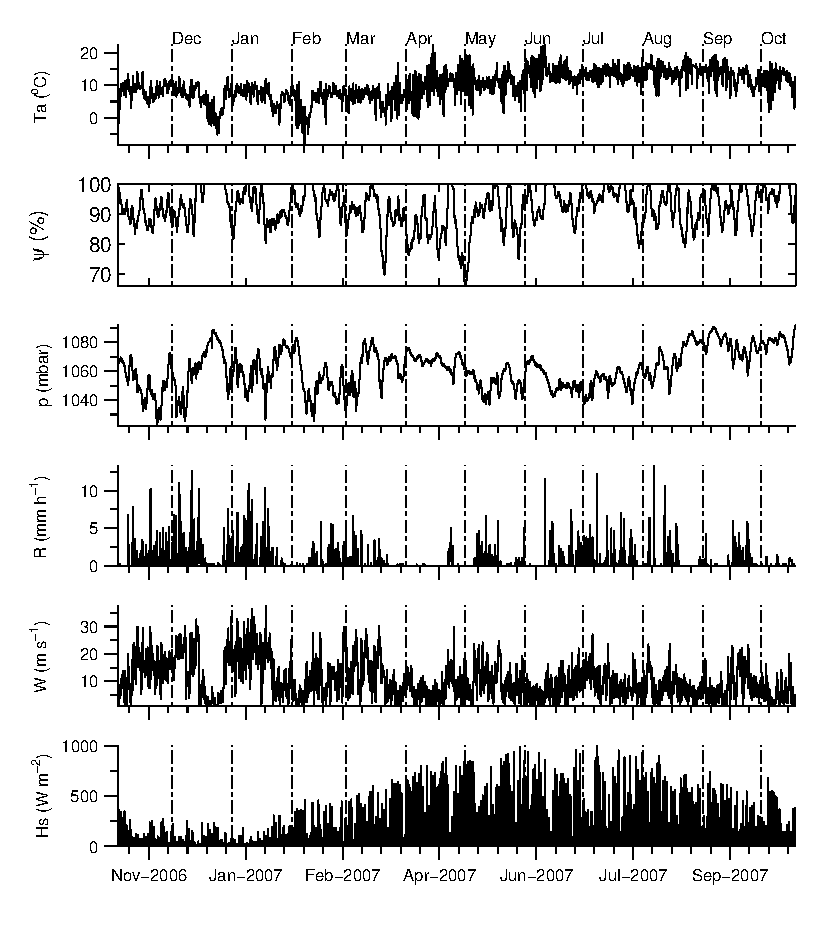
\includegraphics[width=0.4\textwidth]{metVarCaliNew}
    \caption{\tiny Hourly-averaged meteorological data series used in the model calibration. Ta = air temperature; $\psi$  = relative humidity, p = atmospheric pressure; R = hourly rainfall; W = windspeed at a height of 2 m  above the water surface; and Hs = short wave irradiance at the water surface.}
    \label{metVarCali}
  \end{center}
\end{figure}
\end{frame}

\begin{frame}{Calibraci\'on del modelo}
\begin{table}
\centering
\caption{Best parameter set for three different relative water depths ($h/H$) based on the minimum value of $NSE$.}
\begin{tabular}{ccccccc}
\toprule
 h/H & RMSE (m) & RMAE (\%) & NSE & \textbf{$Kz_{max}$} & \textbf{$C$} & \textbf{$\eta$} \\
\midrule 
0 &	  0.688   &	 7.6   &	 0.973  &	 5.60e-05 &	 0.9000 &	 0.3111\\
0.5 &	  0.657  &	6.9  &	 0.971  &	 6.70e-05 &	 0.1000 &	 1.3667\\
1.0 & 	  0.732  &	 8.5   &	 0.963  &	 1.00e-04 &	 0.1000 &	 1.1556\\
\bottomrule
\end{tabular}
\label{paralev}
\end{table}
\end{frame}

\begin{frame}{Calibraci\'on del modelo}
\vspace{-0.2cm}
\begin{figure}[!htbp]
  \begin{center}
      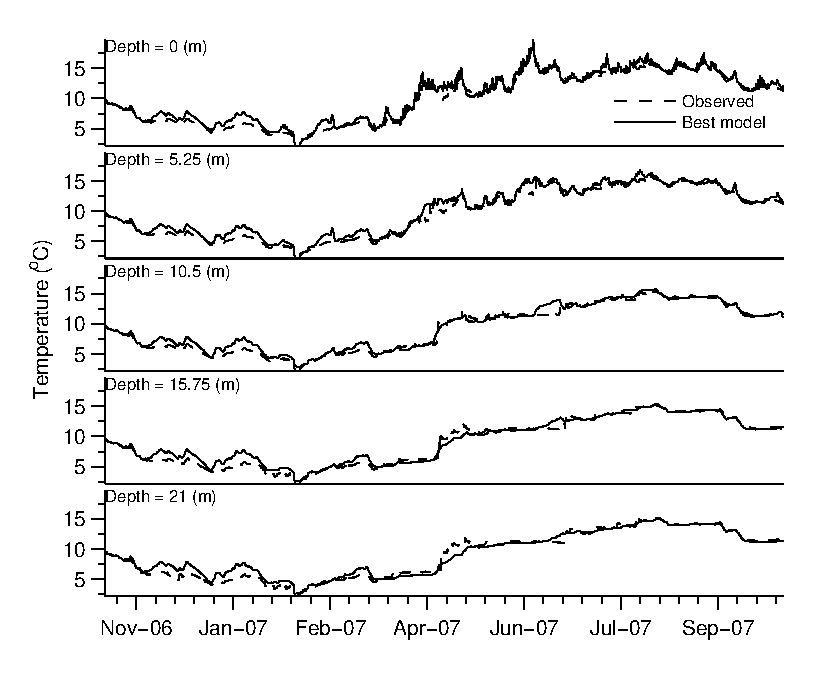
\includegraphics[width=0.55\textwidth]{bestParaNew}
    \caption{\tiny Comparison between simulated and observed water temperature at five depths (every 20\% of the water depth from the surface to the bottom), for the best parameter set  (run 54; Table~\ref{toppara}).}
    \label{bestPara}
  \end{center}
\end{figure}
\end{frame}

\begin{frame}{Validacion del modelo}
\vspace{-0.2cm}
\begin{figure}[!htbp]
  \begin{center}
      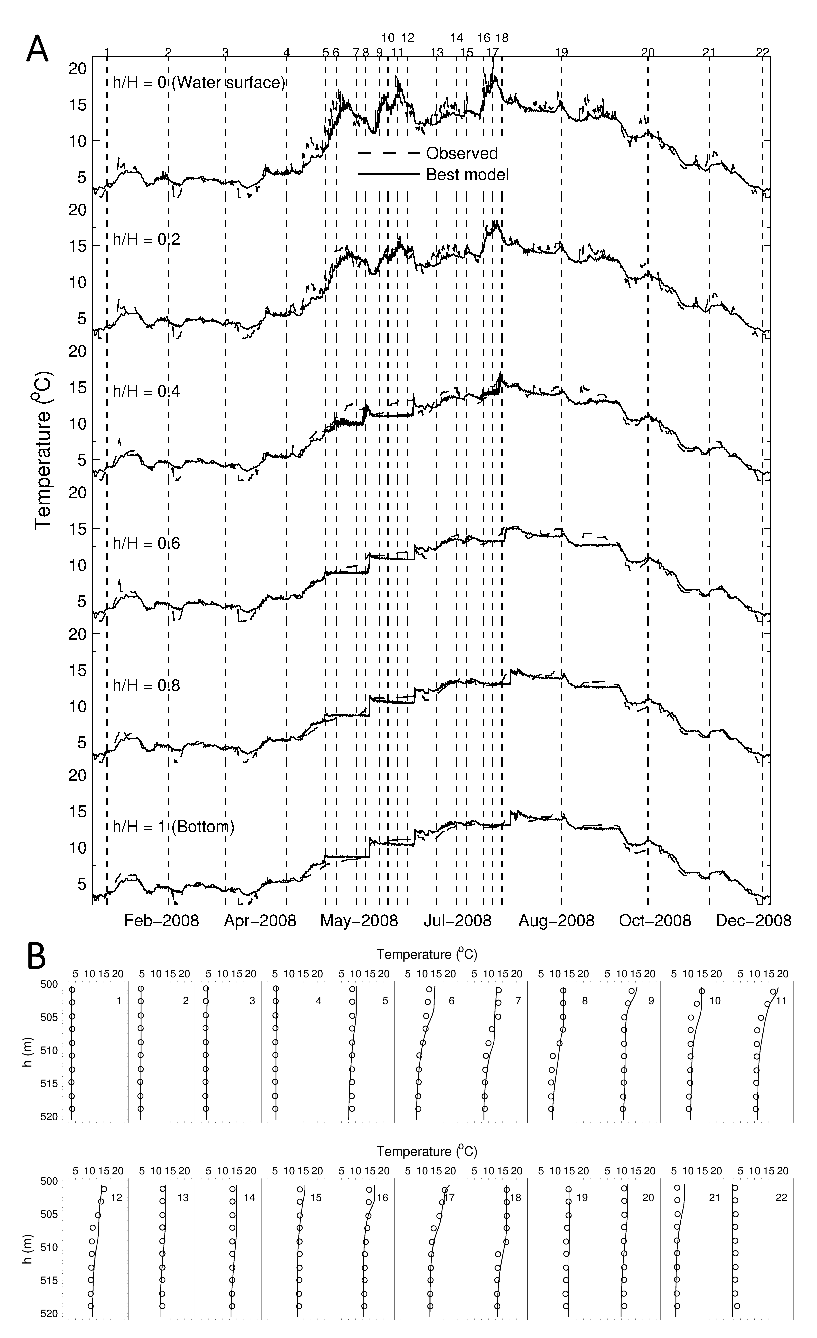
\includegraphics[height=0.74\textheight]{profiAllNewBoth}
    \caption{\tiny a) Comparison between the best simulated (continuous line) and observed temperature (dashed line) at different percentages of water depth from the water surface to the bottom. Vertical dashed lines indicate the times of b) observed (empty circles) and simulated (continuous line) water temperature profiles.}
    \label{profiAll1}
  \end{center}
\end{figure}
\end{frame}

\begin{frame}{Validación del modelo}
\vspace{-0.22cm}
\begin{figure}[!ht]
  \begin{center}
      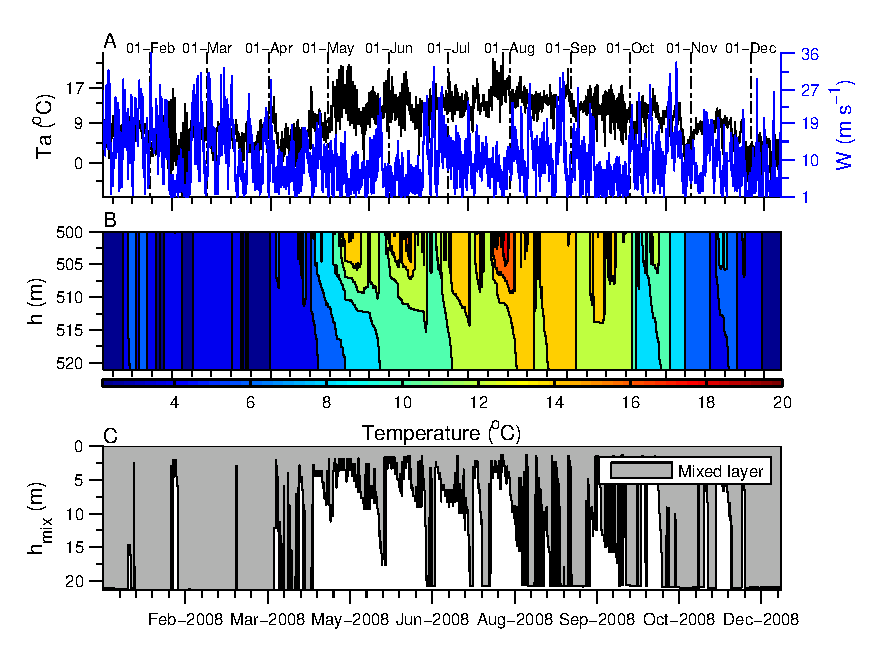
\includegraphics[width=0.63\textwidth]{straAnaNewNew2}
    \caption{\tiny a) Time series for dominant meteorological forcing variables air temperature (black) and wind velocity (blue); b) simulated water temperature contours; c) simulated mixed layer depth.}
    \label{straAna1}
  \end{center}
\end{figure}
\end{frame}

\begin{frame}{Simulacion multidecaadas}
\vspace{-0.4cm}
\begin{columns}
\column{0.5\textwidth}
\begin{figure}[!htbp]
  \begin{center}
      \includegraphics[height=0.75\textheight]{annualWTempDiffLevels}
    \caption{\tiny Multi-decadal UCLake simulation of annual-average water temperature, with 10-year moving average and linear trend for: a) water column average, b) epilimnion, c) metalimnion and d) hypolimnion.}
    \label{annualWTempDiffLevels}
  \end{center}
\end{figure}
\column{0.5\textwidth}
\begin{figure}[!htbp]
  \begin{center}
      \includegraphics[height=0.75\textheight]{seasonalWTemp}
    \caption{\tiny Seasonal water-depth averaged temperature time-series and boxplots for: a) winter, b) spring, c) summer and d) autumn.}
    \label{seasonalWTemp}
  \end{center}
\end{figure}
\end{columns}
\end{frame}

\begin{frame}{Articulo}
\vspace{-0.22cm}
\begin{figure}[!ht]
  \begin{center}
      \includegraphics[width=0.75\textwidth]{arti.png}
  \end{center}
\end{figure}
\end{frame}



%\begin{frame}{Condiciones de frontera}
%The long-wave radiation, $Hl$, is computed as the balance between the radiation emitted by the water surface ($Hl_{ro}$) and the net radiation received from the atmosphere and the clouds, $Hl_{ra}$, given as
%
%\begin{equation}
%	Hl = Hl_{ra} - Hl_{ro}
%\label{Hl}
%\end{equation}
%
%$Hl_{ro}$ is estimated as $Hl_{ro} = \varepsilon_{w} \sigma T_{w}^4$ where $T_w$ is the water surface temperature in $^o$K, $\sigma$ is the Stefan-Boltzmann constant (5.67$\e{-8}$) and $\varepsilon_{w}$ is the emissivity for water ($\sim$ 0.97). $Hl_{ra}$ is estimated from $Hl_{ra} = Hl_{ri}(1 - A_{L})$, where  $A_L$ is the long wave reflectivity constant, which is taken to be 0.03 \citep{henderson1984henderson}. The incoming radiation from the atmosphere and clouds is given by $ Hl_{ri} =\varepsilon_{a} \sigma T_{a}^4$ where $T_a$ is the air temperature in $^o$K and the emissivity $\varepsilon_{a}$ is
%
%\begin{equation}
%\varepsilon_{a} = \left\{ \begin{array}{rl}
% 0.87-\frac{n}{D}(0.175-29.92\e{-6}\psi e_{sa})+2.693\e{-5} &\mbox{ if $\frac{n}{D} \leq 0.4$} \\
% 0.84-\frac{n}{D}(0.100-9.973\e{-6}\psi e_{sa})+3.491\e{-5} &\mbox{ if $\frac{n}{D} \geq 0.4$} 
%       \end{array} \right.
% \label{epsilona}
%\end{equation}
%
%In the above expressions for $\varepsilon_{a}$, $\frac{n}{D}$ is the sunshine duration, and $\psi$ is the relative humidity given as
%$$
%\psi = \frac{\mbox{actual vapour pressure}}{\mbox{saturated vapour pressure}}
%$$
%and the saturated vapour pressure is given by the empirical equation $e_{s} = 2.171\e{10} \exp^{-4157/(T-33.41)}$ (N m$^{-2}$) where $T$ is the temperature of water or air \citep{glanz1973ecologic}.
%\end{frame}
%
%\begin{frame}{Condiciones de frontera}
%The evaporative heat flux, $He$, represents  the heat energy loss due to water evaporation and is determined from
%
%\begin{equation}
% He = L_{v} \rho E;
%\label{He}
%\end{equation}
%
%where the latent heat of vaporisation is given as \citep{huber1968laboratory}  $L_v = 1000[2500.9 - 2.365(T_w - 273)]$ (J kg$^{-1}$). The dependence of water density, $\rho$ (kg m$^{-3}$), on temperature is approximated as $\rho = 1000[1.0 - 6.63\e{-6}(T-277)^2]$ .  $E$ is the evaporative flux (s$^{-1}$), given as $E = f(W)(e_{sw} - e_{a})$ where $f(W) = a + bW$ is a function of wind velocity ($W$), and $a$ and $b$ are constants. UCLAKE implements five different formulae for the estimation of $E$. The default option is the widely used Penman equation \citep{penman1948} $E = 0.44\e{-10}(1+0.437 u_2)(e_{sw}-e_a)$ in m s$^{-1}$, where $e_{sw}$ is the saturated vapour pressure at the water temperature and $e_a$ is the actual vapour pressure at the temperature of the air.
%
%\end{frame}
%
%\begin{frame}{Condiciones de frontera}
%The sensible heat flux, $Hc$, is related to $He$ through the Bowen ratio ($\beta$) \citep{henderson1984henderson} as
%
%\begin{equation}
% Hc = 0.61\e{-3} p He \left( \frac{T_w - T_a}{e_{sw}-e_a}\right)
%\label{Hc}
%\end{equation}
%where $p$ is the atmosphere pressure ($\text{mbar}$) and $T_a$ and $T_w$ are air and water temperature respectively.
%
%Turbulent kinetic energy, $E_k$ due to wind shear \citep{ford1980thermal} is computed from
%\end{frame}
%
%\begin{frame}{Condiciones de frontera}
%Turbulent kinetic energy, $E_k$ due to wind shear \citep{ford1980thermal} is computed from
%
%\begin{equation}
%  E_k = \int_{A_s} C \hat{w} \tau dA_{s} 
% \label{Ek}
%\end{equation} 
%
%where $C$ is a wind sheltering coefficient, $A_s$ is the water surface area (m$^2$) and $\hat{w} = \tau / \rho$ is the friction velocity (m s$^{-1}$). $\tau = \rho_{a} C_D W^2$ is the shear stress, where $\rho_{a}$ is air density (kg m$^{-3}$), $C_D$ is the drag coefficient and $W$ is the wind speed (m s$^{-1}$). The drag coefficient is a function not only of the wind speed, but also of the surface wave conditions \citep{wuest2003small}. In UCLAKE, $C_D$ is determined using the following expression originally derived for oceans  \citep{wu1982wind}
%
%\begin{equation}
%C_D = \begin{cases}
%          1.25W^{-0.5}\e{-3} \quad &W \leq 1 \text{m s$^{-1}$}  \\
%          0.5W^{0.5}\e{-3}   \quad &1. < W < 15 \text{m s$^{-1}$} \\
%          2.6\e{-3} 	     \quad &W \geq 15 \text{m s$^{-1}$} \\
%         \end{cases} 
%\end{equation}
%
%\end{frame}


%
%\begin{frame}{Modelos hydrologicos}
%%\centering
%%\includefigure[]{}
%\end{frame}
%
%\begin{frame}{Modelos hidraulicos e hidrodinamicos}
%\end{frame}
%\begin{frame}{Modelos de calidad de agua}
%\end{frame}
%\begin{frame}{Modelos de gestion del recurso hidrico}
%\end{frame}



\end{document}
